\chapter{Machine Learning}
\label{chap:ml}

This section outlines the basic methodology followed in machine
learning approaches to Natural Language Processing. I will briefly
discuss machine learning from a general point of view and then present
supervised machine learning in more detail using linear regression as
example. I will then elaborate on the different kinds of classifiers
applied in NLP; both unstructured and structured.

\subsection{Overview}
%\begin{itemize}
%\item Rule-based vs. machine learning approaches.
%\item The basic machine learning tasks: classification and clustering.
%\item The basic machine learning approaches: supervised and
%  unsupervised learning.
%\end{itemize}

\paragraph{Statistical and Rule-Based NLP}
Approaches to Natural Language Processing can be broadly divided into
two groups: rule-based and machine learning approaches. Rule-based
approaches utilize hand crafted rules for tasks such as text labeling
or machine translation. Machine learning approaches solve the same set
of problems using data driven (usually statistically motivated) models
and samples from the problem domain, which are used to estimate model
parameters.

This thesis focuses on extending machine learning techniques to the
domain of morphologically complex languages, where they have been
applied less frequent than for morphologically more straightforward
languages like English. I want to emphasize that the thesis should not
be seen as an attack against the rule-based paradigm for Natural
Language Processing which has proven to be very successful in
treatment of morphologically complex languages \cite{}. This thesis is
simply an investigation into extension of machine learning
techniques. Truly successful language processing systems should
probably combine rule-based and statistical techniques.

Machine learning and hand crafted rules have their respective merits
and short-comings and these are dependent on the task to some
extent. For example, in the domain of machine translation, rule-based
methods can give syntactically correct results \cite{}. However,
statistical machine translation systems are in general better at
lexical choice \cite{}.

\paragraph{Supervised and Unsupervised ML}Machine learning is can be
divided into two fields supervised and unsupervised. Supervised
machine learning uses a training material of labeled training
examples. An example would be a set of images with associated key
words, where the task is to build a system which can associate
previously unseen images with appropriate key words.

Supervised machine learning is typically employed for tasks such as
labeling (that is classification) and translation. Typical examples of
tasks include Part-of-Speech labeling and speech recognition where
annotations consist of POS labels for the words in some text and
written sentences corresponding to an acoustic speech signal
respectively.

In contrast to supervised machine translation, unsupervised approaches
exclusively utilize unannotated data. Unsupervised machine learning is
most often used for various kinds of clustering tasks, that is
grouping sets of examples into subsets of similar examples. 

Finally, semi-supervised (and weakly supervised) systems use an
annotated training set with in combination with a, typically, very
large unannotated training set to improve the results beyond the
maximum achievable by either approach in isolation.

In Natural Language processing, supervised learning approaches are
most often used (for example ...). Unsupervised approaches, however,
can also be useful for e.g. exploratory data analysis (...).

This thesis focuses on supervised machine learning.

\section{Supervised Learning}
%\begin{itemize}
%\item Example: linear regression.
%\item Estimation from a sample.
%\item Convexity, smoothness.
%\item Regularization.
%\item Methodology: Training, development and test sets. 
%\item Significance testing.
%\end{itemize}

In this section, I will illustrate the key concepts and techniques in
supervised Machine Learning using the simple example of linear regression. I will explain the plain linear regression model and show how it can be fitted using training data. I will then briefly present ridge regression which is a regularized version of linear regression.

I chose linear regression as example because it is a simple model yet
can be used to illustrate data driven techniques. Moreover, the model
has several tractable properties such as smoothness and
convexity. Additionally, it can be seen as the simplest example of a
linear classifier which is a category of models encompassing

\subsection{Basic Concepts}

\paragraph{Linear Regression} As a simple example, imagine a person
called Jill who is a real estate agent. She is interested in
constructing an application, for use by prospective clients, which
would give rough estimates for the selling price of a property. Jill
knows that a large number of factors affect housing prices but there
are a few very robust quantifiable predictors of price that are easy
to measure.

Jill decides to base the model on the following predictors:
\begin{enumerate}
\item The living area.
\item The number of rooms.
\item The number of bathrooms.
\item Size of the yard.
\item Distance of the house from the city center.
\item Age of the house.
\item Amount of time since the last major renovation.
\end{enumerate}

Jill decides to use the simplest model which seems reasonable. This
model is {\it linear regression} which models {\it the dependent
  variable} house price as a linear combination of the independent
variables listed above and parameter values in $\R$. The linear
regression model is probably not accurate. It fails in several
regards. For example, increasing age of the house probably reduces the
price up to a point but very old houses can in fact be more expensive
then newly built houses especially if they have been renovated lately.
Although, the linear model is unlikely to be entirely accurate, Jill is
happy with it because the intention is just to give a ball park
estimate of the price for the average prospective client.

To formalize the linear regression model, let us call the dependent
variable price $y$ and each of the independent variables living area,
number of rooms and so on $x_i$. Given a vector $x = (x[1], ...,
x[n])^\top \in \R^n$, which combines the independent
variables\footnote{In reality, each of the predictors would probably
  be transformed to give all of them the same average and
  variance. Although this ii not required in theory, it tends to give
  a better model \cite{someone}.}, and a parameter vector $\theta \in
\R^n$ the linear regression model is given in Equation
\ref{eq:linreg}.

\begin{equation}
y(x\parcond \theta) = x^\top\theta\label{eq:linreg}
\end{equation}

Two questions immediately arise: How to compute the price given
parameters and predictors and how to compute the parameter vector
$\theta$. These questions are common for all supervised learning
problems also when using other models than the linear regression
model.

\paragraph{Inference} The first question concerns {\it inference},
that is finding the most likely value for the dependent variable given
the independent variables. In the case of linear regression, the
answer to this question is straightforward. To compute the price,
simply perform the inner product in Equation \ref{eq:linreg}. The
question is, however, not entirely settled because one might also ask
for example how close to the actual price the estimate $y$ is likely
to be. A related question would be to provide an upper and lower bound
for the price so that the actual price is very likely to be inside the
provided bounds. To answer these questions, one would have to model
the expected error.

Inference is very easy and also efficient in the case of linear
regression. With more complex model such as structured graphical
models used in this thesis, it can however be an algorithmically and
computationally more challenging problem. The principle is still the
same: Find the $y$ which is most likely given the input parameters.

\paragraph{Estimation} The second question concerns {\it estimation of
  model parameters} and it is more complex than the question of
inference. First of all, Jill needs training data. She also needs to
decide upon an {\it estimator}, that is, a method for estimating the
parameters $\theta$.

In the case of house price prediction, Jill can simply use data about
houses she has brokered in the past. She decides to use a training
data set $\mathcal{D} = \{(x_1, y_1), ..., (x_T, y_T)\}$, where each
$x_t = (x_t[1] ... x_t[n])$ is a vector of independent variable values
(living area, age of the house and so on) and $y_t$ is the dependent
variable value, that is the final selling price of the house. Now Jill
needs to make a choice. How many training examples $(x_t, y_t)$ does
she need? The common wisdom is that more data is always better,
however, this has bearing on how the parameters need to be
estimated. In any case, the number of data points in the training data
should ideally be higher than the number of parameters that need to be
estimated. When one cannot accomplish this, one encounters the so
called {\it data sparsity problem}.

\paragraph{Data Sparsity} Whereas getting sufficient training data is
fairly easy in the case of housing prices, it is vastly more difficult
to accomplish with more complicated models in natural language
processing. Therefore, one central question in this thesis is how to
counteract {\it data sparsity}.

\paragraph{Cost Functions} The objective in estimation is to find a
parameter vector $\theta$ which in some sense minimizes the error of
the house price predictions $y(x_t\parcond \theta)$ when compared to
the actual realized house prices $y_t$ in the training data. The usual
minimization criterion used with linear regression is the least square
sum criterion given in Equation \ref{eq:lss}. It is minimized by a
parameter vector $\theta$ which gives as small square errors $|y_t -
y(x_t \parcond \theta)|^2$ as possible.

\begin{equation}
\theta = \argmin_{\theta' \in \R^n} \sum_{x_t \in \mathcal{D}} | y_t - y(x_t\parcond \theta')|^2\label{eq:lss}
\end{equation}

The square sum is an example of a {\it cost function} (also
called the objective function). A cost function assigns a non-negative
real cost for each parameter vector. Using the concept of cost
function, the objective of estimation can be reformulated: Find the
parameter vector $\theta$ that minimizes the cost of the training
data.

\paragraph{The Exact Solution} In the case of linear regression, there
is a well known exact solution for $\theta$ which utilizes linear
algebra. The solution is given in Equation \ref{eq:lss-exact}. The
matrix $X \in \R^T_n$ is defined by $X_{t,i} = x_t[i]$ and its
More-Pennrose pseudoinverse $X^+ \in \R^n_T$ is defined as $X^+ =
(X^\top X)^{-1}X^\top$. The vector $Y \in R^T$ is simply the vector of
realized house prices $y_t$. The solution $\theta$ exists only when
none of the independent variables are linear combinations of each
other in the training data.

\begin{equation}
\theta = X^+ Y \label{eq:lss-exact}
\end{equation}

\paragraph{Iterative Estimation} Although the linear regression model
is simple enough so that it can be estimated exactly, the same does
not hold for most more complex models such as the Conditional Random
Field investigated in this thesis. Moreover, the exact solution might
often not be the one that is desired. Often the training data is quite
sparse, that is there is too little of it compared to the amount of
parameters that need to be estimated. Therefore, the model may {\it
  over-fit} the training data and fail to generalize well to examples
not included in the training data. 

\paragraph{Regularization} Due to the problem of over-fitting, a family
of heuristic techniques called {\it regularization} is often
employed. They aim to transform the original problem in a way which
will penalize both deviance from the gold standard and ``complexity''
of the solution $\theta$. Regularization can be seen to convey the
same idea as Occam's Maxim which states that a simpler explanation for
a phenomenon should be preferred when compared to a more complex
explanation yielding equivalent results. Of course, this does not
explain what is meant by a ``complex'' parameter vector $\theta$.

To illustrate simple and complex parameter vectors, examine a case of
linear regression where the dependent variable $y$ and the predictors
$x_i$ have mean $0$ and variance $1$ in the training data. This may
seem restrictive but in fact any linear regression problem can easily
be transformed into this form by applying an affine transformation $z
\mapsto az - b$. When doing inference, this affine transformation can
simply be reversed by applying $z \mapsto a^{-1} (z + b)$. The
simplest parameter vector $\theta$ is clearly the zero vector $\theta
= (0 ... 0)^\top$. It corresponds to the hypothesis that the
predictors $x_i$ have no effect on the dependent variable
$y$. According to this hypothesis, the prediction is always the
average of the dependent variable values in the training data.

The zero solution to a linear regression problem is simple but also
totally biased. Because we are assuming that the independent variables
$x_i$ explain the dependent variable $y$, a model that completely
disregards them is unlikely to give a good fit to the training
data. By introducing a regularization term into the cost function, we
can however encourage simple solutions while at the same time also
preferring solutions that give a good fit. There are several ways to
accomplish this but the most commonly used are so called $L_1$ and
$L_2$ regularization. These are general regularization methods that
are employed in many models in machine learning.

The $L_1$ regularized cost function for linear regression is given in
Equation \ref{eq:lss-l1}. $L_1$ regularization, also called LASSO
regularization \cite{somone}, enforces solutions where many of the
parameter values are $0$. These are also called sparse parameters. It
is suitable in the situation where the model is over specified, that
is, many of the predictors might not be necessary for good prediction. The expression is a sum 

\begin{equation}
\theta = \argmin_{\theta' \in \R^n} \sum_{x_t \in \mathcal{D}} | y_t - y(x_t\parcond \theta')|^2 + \lambda \sum_i |\theta[i]|\label{eq:lss-l1}
\end{equation}

The $L_2$ regularized cost function is given in \ref{eq:lss-l2}. $L_2$
regularization is also called Tikhonov regularization. In contrast to
$L_1$ regularization, it directly prefers solutions with small norm. A
linear regression model with Tikhonov regularization is called a ridge
regression model.

\begin{equation}
\theta = \argmin_{\theta' \in \R^n} \sum_{x_t \in \mathcal{D}} | y_t - y(x_t\parcond \theta')|^2 + \lambda \|\theta\|^2 = \argmin_{\theta' \in \R^n} \sum_{x_t \in \mathcal{D}} | y_t - y(x_t\parcond \theta')|^2 + \lambda \sum_i |\theta[i]|^2\label{eq:lss-l2}
\end{equation}

The coefficient $\lambda \in \R^+$ is called the {\it
  regularizer}. The regularizer determines the degree to which model
fit and simplicity affect the cost. A higher $\lambda$ will increase
the cost for complex models more than a lower one. When $\lambda$
increases, the optimal parameter vector $\theta$ approaches the zero
vector and when it decreases $\theta$ approaches the parameters that
fit the training data as closely as possible. This is called
under-fitting.

The regularizer is a so called {\it hyper-parameter} of the
regularized liner regression model. It is easy to see that increasing
$\lambda$ will automatically increase the cost. Therefore, there is no
direct way to estimate its correct magnitude simply using the training
data. Instead {\it held-out data} can be used. Held-out data is
labeled data that is not used directly for estimating model
parameters. If the model over-fits the training data, that is
generalizes poorly to unseen examples, the held-out data will have a
high cost. However, it will also have a high cost if the model
under-fits, that is, performs poorly on all data. Held-out data can
therefore be used to find an optimal values for the regularizer
$\lambda$. Often one tries several potential values and chooses the
one that minimizes the cost of the held-out data. Usually, one uses
the unregularized cost function for the held-out data.

\paragraph{Iterative Estimation} Regularization is an additional
reason for introducing iterative estimation methods instead of exact
estimation. There are several choices of regularization methods and
some of them might not result in optimization problems that have
closed form solutions\footnote{In the case of regression, non-linear
  {\it kernel functions} also result in optimization problems that
  don't have a closed form solution. I will elaborate this when
  discussing logistic regression.}. When an exact solution cannot be
computed, or it is undesirable, numerical methods can be used to
estimate model parameters.

Because the cost of the training data is a function of the model
parameters, one can apply analytical methods to try to find optimal
parameter values. These methods include for example Newton's method
which is an iterative procedure that can be used to find the zeros of
a differentiable function or local extrema of a twice differentiable
function. Approximations of Newton's method, so called Quasi-Newton
methods \cite{somone}, have also been developed because Newton's
method requires evaluation and inversion of the Hessian matrix of a
function. This is a very costly operation for functions where the
domain has high dimension. Quasi-Newton methods use approximations of
the inverse Hessian. 

A simpler method called gradient descent can be applied to functions
that are only once differentiable.\footnote{Essentially the same
  procedure can also be applied to functions that are not
  differentiable but are only guaranteed to have a sub-gradient
  \cite{someone}.} In general, gradient descent converges toward the
optimum more slowly than Newton's method, however, the computation of
one step of the iterative process is much faster when using gradient
descent. Therefore, it may be faster in practice.

All gradient based methods rely on differentiability of the cost function. For the models used in this thesis, differentiability holds. Gradient based methods work in the following general manner. Let $L_{\mathcal{D}}:\R^n \rightarrow \R$ be the cost of the training data $\mathcal{D}$.

\begin{enumerate}
\item Start at a random point $\theta_0$ in the parameter space.
\item Determine the direction of steepest descent of the cost function. This is the negative gradient $-\nabla L_{\mathcal{D}}(\theta_t)$ at point $\theta_t$.\label{alg:dir}
\item Determine a suitable step size $\alpha_t \in \R_+$. 
\item Take a step of length $\alpha_t$ in direction $v_t$ to get to the next point in the parameter space $\theta_{t+1}$, that is $\theta_{t+1} = \theta_t - \alpha_t \nabla L_{\mathcal{D}}(\theta_t)$.
\item If the difference in cost $|L_{\mathcal{D}}(\theta_{t+1}) - L_{\mathcal{D}}(\theta_t)|$ is smaller than a threshold $\rho$, set $\theta = \theta_{t+1}$. Otherwise, set $\theta_t = \theta_{t+1}$ and return to line \ref{alg:dir}.
\end{enumerate}

The main difference between first and second order methods is the
computation of the step size $\alpha_t$. Second order methods can take
longer steps when the cost is plateauing. Thus they typically take
fewer steps in total. In first order methods such as gradient descent,
$\alpha_t$ can be constant, a decreasing function of $t$ or can also
be determined by a line search in the direction of $-\nabla
L_{\mathcal{D}}(\theta_t)$ \cite{someone}. For example $\alpha_t =
t^{-1}$ may work\footnote{In general, stepsize $(\alpha_t)_{t \in \N}$
  that resemble the harmonic sequence, that is $\sum \alpha_t^2 <
  \infty$ and $\sum \alpha_t = \infty$, guarantee convergence of
  gradient descent to an minimum of the cost function (if it exists)
  for a wide variety of functions \cite{someone}}.


As the meta-algorithm above suggests, gradient based optimization
algorithms are local in the sense that they always move in the
direction of steepest descent of the cost function that is toward a
local optimum. Therefore, they will in general not find the global
optimum of the cost function. By choosing a {\it convex} cost function
it is possible to avoid getting stuck at local optima. All local
optima of convex functions are in fact global optima. 

Convexity is, however, not enough to guarantee convergence to a global
optimum. First of all, a global optimum might not exist\footnote{This
  can happen if the domain of the cost function is not
  compact. Unfortunately, it usually is not.}. Convergence could also
be too slow thus leading to premature termination of the training
procedure. This is specifically a problem for first order methods.

\paragraph{Online Estimation} The optimization methods
discussed up to this point have been so called {\it batch
  methods}. The derivatives of the cost function is computed over the
entire training data and parameters are updated accordingly. Batch
methods can be slow and subsequent training when new training examples
become available is computationally intensive. {\it Online algorithms}
are an alternative to batch methods, where the cost is instead
computed for a randomly chosen training example and the parameters are
the updated accordingly \cite{someone}. In practice, online methods
can give fast convergence. Moreover, re-training is relatively
efficient when new training examples become available.

{\it Stochastic gradient descent} is a well known online estimation
algorithm. It has vastly superior convergence properties when compared
to regular gradient descent \cite{someone} but is identical in all
other respects except that it is an online estimation algorithm
instead of a batch algorithm. The algorithm processes one random
training example at a time. It uses the gradient $\nabla
L_{\mathcal{D}[i]}(\theta)$ of the cost over the single training
example $\mathcal{D}[i]$ to approximate the gradient $\nabla
L_{\mathcal{D}}(\theta)$ for the entire training data $\mathcal{D}$.

\section{Classifiers}
%\begin{itemize}
%\item Naïve Bayes' classifier.
%\item Generative and Discriminative Classifiers.
%\item Linear classifiers: logistic classifier, perceptron classifier \citep{Freund1999},
%  SVM \citep{Cortes1995}.
%\end{itemize}

The main topic of this thesis is morphological tagging. It can be seen
as a structured {\it classification task} where each word in a
sentence is assigned one morphological label\footnote{which may have
  internal structure as is seen in Section
  \ref{sec:sub-labels}.}. Classification is a fundamental supervised
machine learning task where the objective is to learn a mapping from
objects like words, sentences, documents or images onto discrete
classes such as morphological labels (Noun+Sg+Nom) or sentiments
(Positive sentiment versus Negative Sentiment).

Classification resembles regression. The output of a classifier is, however, not
a single real value $y$ but a distribution over the set of nominal
classes.

Probabilistic classifiers can broadly be divided into two groups,
namely generative and discriminative. Generative classifiers learn a
joint distribution $p(x,y)$ over labels $y$ and input examples
$x$. Given an example $x$, a distribution over classes $y$ can be
computed using the marginal probability of example $x$, which is $p(x)
= \sum_{y' \in Y} p(y',x)$. The probability distribution over classes
is defined by $p(y|x) = p(y,x) / p(x)$.

\section{Structured Classifiers}
%\begin{itemize}
%\item The idea of chained stochastic processes.
%\item Markov chain.
%\item HMM
%\item MEMM
%\item CRF
%\end{itemize}

There are tasks in natural language processing that cannot be
adequately formulated as supervised classification tasks in the simple
way that has been discussed earlier. Examples of tasks that require
more sophisticated methods are syntactic parsing and translation
between languages. One could think of parsing as a labeling task where
the objective is to label a sentence with the appropriate syntactic
tree. Likewise, the translation of a sentence could be seen as its
label. 

It is, however, easy to see that these approaches are deeply
flawed. Firstly, there is an infinite number of syntactic trees and
indeed an infinite number of sentences of finite length. Therefore,
the label set would have to be infinite as well. Secondly, the data
sparsity problem would be unmanageable. Just in order to see most
relatively frequent syntax trees for moderately long English
sentences, say twenty words long, we would need an unfathomable amount
of training data.

Instead of a simplistic classification approach, {\it structured}
classifiers can be employed. Structured classifiers relate parts of
the complex label such as a translation, syntax tree or sequential
labeling with the input. They also learn how to piece together complex
labels from simple constituents. A very simple (and probably very bad)
translation software could learn how to translate isolated English
words into French words and then learn how to combine French words
into sentence as shown in Figure \ref{fr-tr}. Note that although both
``Le'' and ``La'' are perfectly good translations for ``The'', only
``Le'' is usually possible before ``chien'', which is a masculine
French word.

In general, structured classifiers rely on two models, the
unstructured and structured model. The unstructured model learns to
relate simple labels such as words in a translation or nodes in a
syntax tree with the input. In contrast, the structured model learns
how to combine simple labels into complex labels such as entire
translations or syntax trees. In practice, some models make a stricter
division then other models.

Structured models are the main subject matter of this thesis and I
will present two structured models, the Hidden Markov model and the
Conditional random field in detail in Chapters \ref{hmm} and
\ref{crf}.
 
\begin{figure}
\caption{A translation from English to French}\label{fr-tr}
\begin{center}
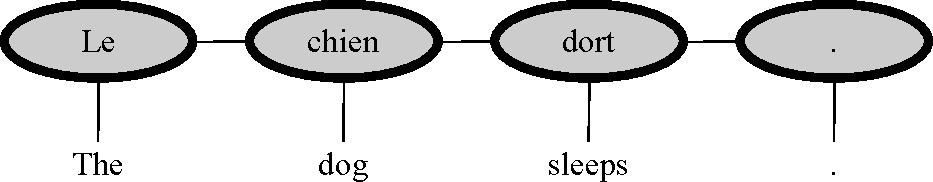
\includegraphics[scale=0.75]{chien}
\end{center}
\end{figure}

\section{The Aim of Research -- Improving the State of the Art}

Like most language technological research, the work documented in this
thesis aims at improving existing solutions for language
processing. Specifically, my work is targeted at improving
morphological taggers for morphologically rich languages. It is not
entirely easy to define what constitutes an improvement to the field
of morphological tagging or indeed any sub-field of language
technology. Nevertheless, most researchers would probably agree that
the following kinds of changes are improvements compared to existing
approaches:

\begin{enumerate}
\item Improving labeling accuracy.
\item Speeding up estimation.
\item Speeding up tagging.
\item Reducing model size. \label{quant}
\item Clarifying the underlying theoretical foundations.
\item Simplifying implementation of taggers.
\item Uncovering best practices for building taggers.
\end{enumerate}

Items 1 though \ref{quant} in the list above are {\it quantifiable}
improvements. It is possible to perform experiments to measure the
labeling accuracy, tagging speed, estimation speed and model size
given by different morphological taggers and derive conclusions about
the respective merits of the taggers. In contrast, the rest of the
items in the list cannot be measured as easily. 

Although, most probably would agree that clarifying theoretical
foundations of a field is a substantial contribution, it may not be as
easy to agree upon what constitutes a clarification. This could for
example be dependent on the background of individual
researchers. Similarly, one model might be more straight-forward to
implement than another model using some programming language, however,
this can very well depend on the specific programming language and
available libraries to some degree.

Because quantifiable improvements are easier to ascertain, this thesis
focuses on demonstrating such improvements compared to other state of
the art approaches. Nevertheless, I will also aim to show that the
model demonstrated in the thesis is conceptually simpler than other
state of the art approaches.

Although quantifiable improvements are easier to demonstrate than
other improvements, there are still caveats. First of all, it is
impossible to compare machine learning models directly. One can only
compare implementations of the models. Because of differences between
platforms even different implementations of the exact same model can
have radically different run time on the same data. Moreover, bugs in
the implementation of different models can reduce the accuracy or have
sporadic effects on run time.

Besides practical concerns like dependence on implementation, there
are also theoretical issues that interfere with measuring performance
of different models. It is easy to say that the accuracy of one system
is better than another system on {\it a specific data set}. This does,
however, not imply that the accuracy is better on {\it all data
  sets}. In formal terms, we can only conduct experiments on samples
of the distribution of all texts in a given language. Therefore, our
experiments will yield results only in a probabilistic sense: it is
likely that the labeling accuracy of one system is better than the
accuracy of another, if the accuracy was better on the sample used for
testing.
 
Using large test sets and test sets compared from a variety of
different genres will probably give more reliable results. This is,
however, also to some extent a debatable matter. Some methods are very
accurate on the same genre that they were trained on but perform worse
on other genres. Other methods instead perform well on average but, as
a trade-off, cannot reach as high accuracy on a specific text
domain. It is not easy to say which kind of system is preferable. This
trade-off is called the bias variance trade-off \cite{?} and it has
bearing on measuring the performance difference of systems. 

When using a high variance system, accuracy on different texts varies
a lot. When instead using a system with high bias, the accuracy tends
to vary much less.

When comparing two systems, it is not sufficient to simply look at the
performance of the systems on a test set. If we measure the
performance of the systems on a particular test, one of them will
almost certainly perform better than the other regardless of whether
there is an actual difference in the performances of the systems. The
probability of exactly equal performance is simply very small. 

The larger the test sets are, the more accurately the results of
experiments will on average reflect the true performance of the
systems. This is easy to see, because ultimately the test set will represent the entire domain. Unfortunately, the amount of test material is usually
restricted and producing more test data might not be
feasible\footnote{Especially when using standard data sets, one is
  restricted to the given amount of test data}.

An approach that is often used is splitting the test data into
segments and performing several experiments -- one for each
segment. If one system outperforms the other system on most segments
with a large margin, then we are more confident in saying that there
is in fact a difference in the performance of the systems. If on the
hand each system outperforms the other on roughly half of the
segments, we might be inclined to doubt whether there is any real
difference in performance between the systems. The higher the variance
between the results, the larger the margins between the systems need
to be in order for us to be able to conclude that there is a
difference in performance. This argument can be made rigorous using
statistical tests which measure the significance of the difference in
performance of two systems.

The usual set up of statistical significance testing is to make a null
hypothesis $H_0$ that the average performance of two systems is the
same. After this a test statistic is computed. The test statistic is
simply a real number whose value indicates the significance of the
difference in performances between the systems. If the statistic is
high enough, the null hypothesis can be discarded in favor of the
alternative hypothesis that there is a genuine difference in
performance between the systems. The test statistic incorporates
information about the difference in performance of the systems on test
data all segments as well as the variance of the performances.

In the work conducted presented in this thesis, I have used the
Wilcoxon signed-rank test \cite{?} to ascertain the significance of
results. I use it instead of the T-test because it is not dependent on
the fact that the distribution of differences in performance are
normally distributed\footnote{In practice it might be a fairly
  accurate assumption that the differences are normally
  distributed. This often holds for measurements \cite{?}.}. In
practice it is less sensitive than the T-test.

